
\renewcommand{\thefootnote}{\arabic{footnote}}

\chapter[G Ramachandran– A tribute]{G Ramachandran– A tribute\footnote{Parts of this account was originally written as a 80th birthday felicitation. GR actually read it and commented on it pointing out some inaccuracies which have been corrected (or commented) in this version.}}\label{chap14}

\Authorline{M V N Murthy}



GR, as we referred to him, was one of the founding members of my place of work, The Institute of Mathematical Sciences. He along with other members of the Theoretical Physics Seminar Group formed the core of Matscience (as IMSc was called then) when it began in 1962. GR had an illustrious career in Theoretical Physics for nearly six decades without a break during which he made many significant research contributions, guided more than twenty researchers for their doctoral degrees and, most importantly taught a huge number of students at the University of Mysore and many other institutions with which he was associated. There are very few academics in India (or any where else for that matter) who have carried their good work in teaching and research for as long as GR (as we always referred to him) has done and was still going strong at the time of his passing away.

first met GR in 1973 in Mysore\footnote{In actual fact I met him a year earlier in Central College, Bangalore. GR had been invited to deliver a lecture in the Physics Association and I had gone to IISc to meet him in this context. I had forgotten this and it was GR who reminded me last October when we exchanged some emails}. GR joined the faculty of the Department of Physics, University of Mysore in 1973 when I was in my second year of MSc specialising in Theoretical Physics. The physics department in Mysore was well known at that time and I moved there for masters after doing physics honours in Central College, Bangalore. It was a breath of fresh air after Central College where the teaching, with one or two honourable exceptions, was almost non-existent. University of Mysore was one of the few universities in India at that time to offer a specialisation in Theoretical Physics and that was the reason I moved there from Bangalore. The department was reasonably big with more than twenty faculty members. Before GR joined, theoretical physics was taught by Professors K N Srinivasa Rao (KNS), A V Gopala Rao (AVG) and one more person who was not cut out for teaching theoretical physics. Other courses, in both years, also had many brilliant teachers.

KNS taught us Classical Mechanics in the first year and, Linear Algebra and Group theory in the second year. AVG taught us Tensor Analysis and General Theory of Relativity. Both KNS and AVG were brilliant teachers, with enormous attention to rigour, a hall mark of the Mysore school for a long time. However, their research interests as well as teaching was more focused on classical fields as well as Mathematical Physics. In earlier years the course suffered because of a lack of sufficient attention to Advanced Quantum Mechanics and almost total absence of Quantum Field Theory in its curriculum. We learnt some basic Quantum Mechanics in the first year and through a general course in the second year. While we did get good exposure through these courses, they were not adequate for a career in Theoretical Physics. GR’s arrival filled this lacuna. He taught us Advanced Quantum Mechanics and foundations of Quantum Field Theory. While he gave attention to mathematical details, he was also more physical in an intuitive sense in his approach to teaching.

As students we knew about his arrival well in advance since it was much discussed among the faculty. It was rather rare to hire a complete outsider as a member of faculty, over looking the claims of local faculty members\footnote{Interestingly, there was no concept of promotion to higher grade. Even local faculty had to compete with others in a selection interview.} , in most state universities. It was even more surprising since the post was that of a Reader and not a lecturer. Most hirings at that time, perhaps even now, were from a pool of former students of the department who either completed their Ph.D while teaching or were hired immediately after their Ph.D. Inbreeding was a very common practice. While inbreeding may be justified for maintaining continuity in laboratory activities, teaching suffered enormously when this tendency became too exclusive. The only honourable exceptions, of hiring from a larger pool, occurred when many physics departments were still in infancy in early sixties. It was very rare to hire rank outsiders in well established departments which had their own internal supply chain. Surprisingly, and to the credit of the head of the department at that time, the physics department in Mysore hired not just one, but three rank outsiders within a span of one year. One of them was GR.


The inevitability of GRs arrival immediately sent a message about his reputation. We came to know that he was a founding member of the Theoretical Physics Seminar led by Alladi Ramakrishnan which became the fountainhead for the creation of the Institute of Mathematical Sciences in 1962 or simply Matscience as it was called in those days. He was later a faculty member at the reputed Indian Statistical Institute in Calcutta headed by the famous statistician C R Rao staffed with a galaxy of future famous mathematicians S R S Varadhan, K R Parthasarathy, V S Varadarajan and Ranga Rao. Later we came to know that GR had to leave ISI and Calcutta under excruciating circumstance in the late sixties. The Naxalite movement impacted the education system so badly that GR’s children could not go to school for a couple of years. Many academics, including a large number from ISI, were forced to leave Calcutta for opportunities else where in the country and abroad. Before coming to Mysore he was a visiting faculty at the Molecular Biophysics Unit(MBU) at IISc working with renowned physicist G N Ramachandran. These famous names like C R Rao or G N Ramachandran added to the aura surrounding GR. Later when I was doing Ph.D, I was helped by many students of MBU who did it simply because of their high regard for GR. Many of these students had benefited by interacting with GR when he was at MBU.

GR’s teaching, though unusual, only enhanced the reputation with which he began his career at Mysore. He usually arrived in the department rather late, after around 11 in the morning or so unless otherwise required. In general his lectures started after lunch in the afternoon when we did not have lab work. More often than not, the lectures would continue for two to three hours. The longest single stretch being about five hours one day, a record of sorts. It was very tiring for us as we were not used to such long sessions. I do not remember GR ever complaining about being tired. We were also fortunate that he, much like KNS and AVG in our senior year, encouraged discussions during and well after these long sessions. During my second year I prepared lecture notes on Scattering theory with his help which he wanted to make copies and preserve. Unfortunately such things were not in vogue nor was it particularly encouraged in the department.

Towards the end of my second year in MSc, I had decided to work with GR for my Ph.D but was not sure that he would accept me as his student. Some time after the exams were over, I asked him if I could work with him. He readily agreed and so I became his research student. He asked me to apply for the CSIR junior research fellowship (JRF). I was joined by R S Keshavamurthy who was also in my class taught by GR. We were both awarded the CSIR JRF starting from January of 1975. Soon we were joined by K Venkatesh a year or so later who came to Mysore after spending a couple of years at Matscience. The three of us parked ourselves in the large room occupied by GR. We put some tables and chairs near the door separating us from GRs work space by a screen of sorts. In fact when it was only Keshavamurthy and me, we used to be described light heartedly as Door Keepers (Dwarapalakas) for GR. For the next five years it was an intense learning experience with GR until the time when I had to leave, rather reluctantly, after my Ph.D and after spending a year as a lecturer, albeit temporary in the department.
\begin{figure}[H]
\centering
\includegraphics[scale=0.27]{src/images/chap14/001.eps}
\caption{GR with his students Keshavamurthy, Ravishankar, he was still in college at this time, and Murthy some time in 1978.}\label{chap14-fig001}
\end{figure}

When I began my research, GR assigned both Keshavamurthy and me to work on the photo-production of pions on deuteron target. The topic of photoproduction of pions on nucleon target was a hot topic in early fifties involving both electro-magnetic and strong interaction. In the absence of a first principle calculation of the process, the phenomenological probability amplitude was formulated by Chew, Goldberger, Low and Nambu, the so called CGLN amplitudes\footnote{G. F. Chew, M. L. Goldberger, F. E. Low and Y. Nambu, Phys. Rev. 106, 1345 (1957)} . Basically, applying symmetry principles as applicable they reduced the number of independent parameters which would then be determined from the experimentally measured cross-sections. At photon energies in excess of a few hundred MeV this process dominates due to resonant cross-section.

In the late fifties, GR and V Devanathan at University of Madras started looking at photoproduction of pions on nuclei, especially the deuteron. The twin objective was to provide more targets, especially since the deuteron is used as a target for neutron (in the absence of free neutron targets) and to also examine nuclear structure through these processes. GR and his collaborators started the pioneering work of using particle probes to study nuclear structure in late fifties and early sixties. In some sense this was the beginning of what came to be later known as Medium Energy Physics (as opposed to High Energy Physics). This is a field that straddles both Nuclear Physics and Particle Physics with know how required from both.

However, around the time I started working on this problem, the field had become some what stale though many people were still active in the field. In part the reason was that the field was too phenomenological depending on experimental inputs for amplitudes at every stage. This “reverse engineering” of sorts is a very difficult art at best. Unfortunately, even to this date it has not changed much since we do not know how to calculate these amplitudes in the non-perturbative regime of the fundamental theory which is Quantum Chromodynamics (QCD).

GR took us through the detailed calculations which involved lot of angular momentum algebra. One of the references we used was the “Lectures on Angular Momentum” (Matscience Report 2, 1963) by GR delivered at Matscience. It was the second such in the lecture notes series, the first being by given by Niels Bohr\footnote{According to GR, chronologically his lectures were delivered first and then by Niels Bohr though they were numbered in the reverse order.} I learnt reasonable amount of quantum theory of angular momentum while working on this problem though I was not too excited about the work I was doing; even to the extent of losing interest in research. I even thought of quitting and changing fields influenced by some brilliant students in economics and philosophy of science. Our work progressed further only because of the hard work by Keshavamurthy and GR’s persistence. The calculations also involved serious numerical computations. We were helped in this by the students of MBU in IISc even though it was frowned upon by some of the faculty members there. More than me, I remember Keshavamurthy carrying huge packs of computer cards to Bangalore every time a calculation had to be done. Even if one card is punched wrongly, the ‘job’ as it was called then had to be submitted again at a counter in the IISc computer center; often requiring another trip to Bangalore.

Fortunately, while I had already spent a year or more working on this problem, two things happened which brought my enthusiasm for research back. The first event took place when GR was visiting the Center for Theoretical Studies (CTS) at IISc in the summer of 1976. Since my parents lived in Bangalore, I also tagged along GR to CTS. Thanks to N Mukunda (who was the chair of CTS) this became an annual summer activity of mine. GR introduced me first to another visitor, K V L Sarma from TIFR and later to S K Singh from IIT Kanpur\footnote{later he moved to his alma mater Aligarh Muslim University after a few years at Jiyaji Rao Scindia University in Gwalior.}. This in itself was unusual since many advisors especially in universities those times, perhaps due to lack of self-confidence or belief in self-worth or simply extracting ‘slave labour’, tended to guard their students from outside influences. Broad collaborations across institutions were rather rare in universities. As for me, these collaborations first with K V L Sarma and later with S K Singh, took me away from my comfort zone in Mysore. I was introduced to the research environment in TIFR and CTS and else where. It was GR’s confidence and broad minded approach to research that allowed these collaborations to happen and flourish even after I obtained my Ph.D.
\begin{figure}[H]
\centering
\includegraphics[scale=.8]{src/images/chap14/002.eps}
\caption{Photograph taken after I left Mysore in GR’s office in 1982: Standing from left to right-S.B. Patangi (student of GR), A.V. Gopala Rao, R.S. Keshavamurthy, V. Ravishankar and R.S. Somashekar (student of D Krishnamurthy and later faculty in the same department)}\label{chap14-fig002}
\end{figure}

These collaborations also introduced me to fields that were new and cutting edge then. Around this time the Standard Model of Particle Physics was just getting formulated. In fact it was known simply as Weinberg-Salam (WS) Model of electro-weak unification at that time. Many parts of the WS model were unverified yet and a lot of work was going on around the world. Together with KVL and GR, I started working on a problem of proposing processes to experimentally determine one of the model parameters, the so called the isoscalar axial vector coupling, that was predicted by the model to be identically zero in the leading order. Such an experiment would constitute a severe test of the WS theory. KVL was thinking of using neutrino scattering on Helium target which was spin zero and isospin zero nucleus hence appeared to be ideal. As it turned out the quantum numbers were not favourable to test WS model since spin polarization asymmetry was identically zero as it should be. This obvious fact was pointed out by GR, and also by Mukunda during our interaction in CTS.

GR then resurrected the proposal by suggesting that we look at the the scattering of neutrinos elastically on a polarised deuteron target (coherent scattering). Deuteron is a spin one target which can be polarised. Since deuteron is also an isoscalar nucleus, any non-zero difference in the rate between deuterons polarised in different states would indicate a non-zero value for the isoscalar axial vector coupling and hence violation of WS theory. Since neutrinos interact only through weak interactions there is no other large background to the process that may arise from electromagnetic or strong processes even though the event rates are extremely small. While the paper was immediately published\footnote{Neutrino scattering on polarised deuterons M.V.N. Murthy, G. Ramachandran, K.V.L. Sarma Pramana 9 (2), 119-127, 1976}, the proposal, though clean, was a far cry from what was feasible experimentally at that time. However, as I was told by some experimentalists, it is the theorists job to propose and leave it to the experimentalists to dispose. For one, detecting neutrinos after scattering is next to impossible then and even now. So the recoil of the final state nucleus has to be measured which is actually tiny in the coherent scattering.\footnote{Coherent neutrino scattering on nuclei was experimentally observed only recently on Cesium. See for example D. Akimov, J. B. Albert, P. An et al., Observation of Coherent Elastic Neutrino-Nucleus Scattering, Science, vol. 357, no. 6356, pp. 1123–1126, 2017.} More importantly, for me, this paper began my life long interest in the field of Neutrino Physics.


A year or so later, with GR and S K Singh, we revisited these calculations in the context of elastic electron-deuteron scattering which was eminently doable. Unlike the neutrino scattering, here both electrons and deuterons can be polarised giving a much better handle on checking the WS model. We looked at all aspects of this process by including the effects of polarisation of electrons, deuterons. Elastic scattering of electrons on polarised deuteron was published in Physics Letters\footnote{Parity violation in polarised electron deuteron scattering MVN Murthy, G Ramachandran, SK Singh Physics Letters B 81 (2), 129-131 (1979)}, and as we were finalising the larger paper, the most definitive confirmation of the Weinberg Salam Model happened when SLAC collaboration announced the results on the measurement of asymmetry in polarised electron-deuteron inelastic scattering, a process on which S K Singh had already published some results a year earlier.

Apart from the tests of Salam-Weinberg model (or Standard Model in today’s jargon), the second set of ideas that enthused me was related some thing that was close to GR’s interests. This is regarding the representation of the density matrix of arbitrary spin systems. He began thinking about this even while he was at Matscience in collaboration with late R K Umerjee. For a statistical assembly of particles with arbitrary spin s, the density matrix may be represented as a $N \times N$ hermitian matrix where the dimension of the representation is $N = 2s + 1$ with its trace equal to unity-
$$
\rho =\dfrac{1}{2s+1}\left[I + \sum\limits_{i=1}^{N^{2}-1} c_{i}O_{i}^{\dagger}\right];\quad Tr(O_{i}O_{i}^{\dagger}) - (2s +1)\delta_{ij}; \quad c_{i}=Tr(O_{i\rho})
$$

where $c_{i}$ are complex numbers which in suitable combination determine spin polarization of the system. The traceless matrices $O_{i}$, $i = 1 \cdots N^{2}-1$ are chosen such that they form an orthogonal basis.

For a spin half assembly, the standard choice is the Pauli matrices. For higher spins the standard choice of basis was the spherical tensor basis (or the Cartesian basis which was even more cumbersome) describing polarisation of
higher spin targets and beams.
$$
\rho= \dfrac{1}{2s+1}\left[I + \sum\limits_{k=1}^{2s}\sum\limits_{q=-k}^{k}(-1)^{q}t_{q}^{k}T_{k}^{q}\right]; \quad t_{k}^{q}= Tr(\rho T_{k}^{q})
$$

The spherical tensor basis $T_{q}^{k}$ , used widely in polarisation physics, are homogeneous polynomials of degree $k$ in terms of the components of the spin vector $\vec{S}$. They transform as tensors under the action of higher dimensional irreducible representations of the rotation group, hence the name spherical tensors. They also form a $N^{2}-1$ dimensional Lie algebra. While the construction of these tensors in the basis is straight forward, it is cumbersome as we go to higher spins.

It was GR’s idea to use the generators of self or fundamental representation of the group SU($N$) instead of the tensors built on higher dimensional representations of the rotations group as the basis for expanding the density
matrix. The set of generators of the group SU(N) can be mapped to the set of spherical tensor when $N = (2s + 1)$ to provide a convenient basis. The Lie algebra ensures that it is an orthogonal basis. For example the spherical tensor basis of a spin half system is mapped on to the three generators of SU(2) which is well known. This was generalised to arbitrary spin s density matrix represented in terms of the $N^{2}-1$ Hermitian generators of the group SU($N$). Thus we wrote
$$
\rho = \dfrac{1}{N}\left[I + \sum\limits_{\alpha-1}^{N-1}h_{\alpha}H_{\alpha} + \sum\limits_{\alpha=1}^{N-1}\sum\limits_{\beta=\alpha+1}^{N}\sum\limits_{\gamma=1}^{2} e_{\alpha \beta}^{\gamma}E_{\alpha \beta}^{\gamma}\right]
$$

where $H_{\alpha}$ are the $N-1$ diagonal generators (which form the Cartan sub-algebra) and $E_{\alpha\beta}$ are in general off-diagonal with zeros along the diagonal. A standard choice is the generalisation of Gell-Mann matrices of SU(3) representation
\begin{equation*}
(H_{\alpha})_{\mu\upsilon} = \left[\dfrac{N}{\alpha(\alpha + 1)}\right]^{1/2} 
\begin{cases} 
& \delta_{\mu\upsilon}\; if\; \mu < \alpha + 1\\
& -\alpha \delta_{\mu\upsilon}\; if\; \mu=\alpha + 1\\
& 0\; if\; \mu > \alpha + 1 
\end{cases}
\end{equation*}
\begin{align*}
(E_{\alpha \beta}^{1})_{\mu\upsilon} &= \sqrt{\frac{N}{2}} \delta_{\mu \alpha} \delta_{\upsilon\beta} = (E_{\alpha \beta}^{1})_{\upsilon \mu}\\
(E_{\alpha \beta}^{2})_{\mu\upsilon} &= -i\sqrt{\frac{N}{2}} \delta_{\mu \alpha} \delta_{\upsilon\beta} = (E_{\alpha \beta}^{2})_{\upsilon \mu}^{\ast}
\end{align*}

Furthermore, as before
$$
h_{\alpha}= Tr(\rho H_{\alpha}), \; e_{\alpha \beta}^{\gamma}= Tr(\rho E_{\alpha\beta}^{\gamma}).
$$

 The Lie algebra of the SU(N) generators may be mapped on to the algebra of spherical tensors for $N = 2s+1$. I liked the approach and immediately started working on SU($N$) representation of polarisation parameters. We first worked on the spin 1 generalisation from spin half and subsequently generalised to arbitrary spin systems.\footnote{A new representation for the density matrix, G Ramachandran and M V N Murthy, Nucl.Phys. A 323, 403-412, (1979)} 

Quite apart from the representation, one of the first things that GR did was to classify the spin systems as \textit{Oriented} and \textit{Non-oriented}. Since the density matrix is hermitian it can always be diagonalised by a unitary transformation. However, if it can be diagonalised by rotations alone, we called them \textit{Oriented Systems}. Such a system can be characterised by an orientation in space involving two angles and $N-1$ real parameters of the density matrix which is now diagonal. Hence an Oriented system is characterised by $N+1$ real parameters. In general an arbitrary spin system involves $N^{2}-1$ parameters and can not be diagonalised by rotations alone. hence it is referred to as \textit{Non-Oriented}. Interestingly, $N=2$ (or spin half) is a special case since the system is always oriented. This is expected since there is only one polarization parameter (vector polarisation) that can be defined for a spin half system.

In a subsequent work,\footnote{A new representation for the density matrix: (II). Equations of motion, G.Ramachandran and M.V.N.Murthy, Nucl. Phys. A337, 301-312 (1980).} we also found that the simplicity of the representation lends itself very well to solve the time evolution or equations of motion of the polarisation parameters. Here we used the power and simplicity of the Lie algebra of the group SU($N$). The SU($N$) representation may be thought of a \textit{normal mode decomposition}, in the sense many coupled equations in spherical tensor basis are decoupled leaving us to solve the equations of motion using a set of lower dimensional (essentially 2$\times$2) matrices. Towards the end of my stay, after K S Mallesh joined our group, we also provided an alternative to Stokes parameters, which describe the polarisation of light, in terms of SU(3) representation of the polarisation of light\footnote{SU(3) representation for the polarisation of light, G Ramachandran, M V N Murthy and K S Mallesh, Pramana 15, 357-369 (1980)}.

In a broad sense the spin physics, of which the above is a part of, became the central theme of many a theses to come out of GR’s group in Mysore. Later this was developed far beyond what we did at that time by GR and his large group of students and collaborators. The first part of my Ph.D thesis essentially consisted of the SU($N$) representation of polarisation and the second part was devoted to the analysis of processes to test the Electro-Weak Model of unification again using polarisation measurables and their sensitivity to model parameters.

Curiously, when I wrote my thesis and gave it to GR in the beginning of 1979, he kept it aside for a few months. Perhaps he was not sure if it was enough. I knew that he did not fully approve of my style of presentation instead of approaching the topic directly, tersely as he would have liked, my approach was perhaps a bit expansive and verbose. In any case the delay came as a blessing since in the intervening period I completed the paper on the equations of motion of polarisation parameters using SU(N) representation and added one more chapter to the thesis. V Ravishankar, who was still a college student a very bright one at that and later to become a member of GR,s group, helped me with many critical comments and corrections.

Towards the end of the year, I mustered enough courage to ask him if I could submit the thesis. He simply asked me one question: “Are you confident of submitting your thesis?”. When I said yes some what blindly, he told me to go ahead and submit the thesis which I did on November 2, 1979 to be precise.\footnote{In an exchange with GR last year, I realised that GR and I have very different recollection of this event. When I gave my thesis draft in February, I still had my fellowship till December. GR thought that I may want to extend my stay till the end, submission early meant an end to the fellowship, to explore the possibility of a faculty position in the department. While it is true that I would have liked to stay on if a possibility existed, I was realistic about its chances being close to zero in the prevailing circumstances.} To me this was a huge confidence building event which was further buttressed when positive reports came. I remember very well when the first report came, I took it to GR at home. He was busy with his morning ritual puja. He did not open it, but kept it for a few minutes in front of the deities before opening and just smiled as he came out. 

Even after my Ph.D, I wrote two more papers in collaboration with GR-one with Ravishankar on the topic of nuclear parity violation and another one with GR and S K Singh on configuration mixing in Carbon nucleus. Later, my interests shifted considerably from Spin Physics. I started working on quark models, perturbative QCD and finally coming back to neutrino physics. However through some discussions with GR and his students I kept up a healthy interest for some time until I lost touch with the work done by his group in later years. GR also broadened his interests in completely different directions. He has trained a large number of students, many of whom are now faculty members in various institutions, universities and colleges in India. More importantly a sizable number of teachers in colleges have obtained their Ph.D working with him either full time or part time. Given the atmosphere in the university departments, ridden with politics and intrigue, what he has achieved through his teaching and research during his tenure and well beyond his retirement from Mysore University is quite remarkable. There are very few who have contributed to teaching and research at his level in any Indian University.

At a personal level, I consider myself fortunate that I was trained by GR in my formative years. His rigorous methods and attention to detail have helped me obtain clarity in my own work even though my approach to physics and research after I left Mysore underwent considerable change, influenced first by K V L Sarma, S K Singh and later by R K Bhaduri. Outside of academics, our views on various things were very different. GR was a religious person with a deep spiritual bent. On the otherhand I kept myself far away from any thing to do with religious pursuits. I also do not think he approved of my participation in many campus left-leaning political activities. Even within the physics department, he kept himself aloof from controversial issues and focussed entirely on teaching and research. He never hankered after power even refusing to become the Chairman of the department, a coveted and powerful position. It is to his credit that none of the differences we had outside of academics came in the way of our academic interaction.

For all that GR has done to me and many students and teachers who came in contact with him over nearly four decades, we all owe him a deep debt of gratitude. The inaugural plaque in front of Matscience has an inscription ”Science is best done when it is a way of life”-that is how GR lived his life.

\begin{figure}[H]
\centering
\includegraphics[scale=1.5]{src/images/chap14/003.eps}
\end{figure}
